For the purpose of understanding different implementations of the same neural network,
we are going to use the previously created CNN classifier and tweak some of its parameters 
to see how the new versions compare with the original one. These modifications include:
\begin{itemize}
    \item Different Architecture
    \item Different Optimizer
    \item Different Normalization Values
    \item Different Activation Functions
\end{itemize}
All test are going to be run for 50 epochs.

\subsection{Different Architecture}
Instead of Convolutional Neural Network, we are going to use a Multi-Layer Perceptron (MLP)
architecture with 3 hidden layers.\\ 
Some information about the two architectures:
\begin{itemize}
    \item \textbf{MLP:} They are composed of perceptrons arranged in multiple layers. They are
    fully connected meaning that each neuron in one layer connects with every neuron in the next
    layer. 
    \begin{figure}[H]
        \centering
        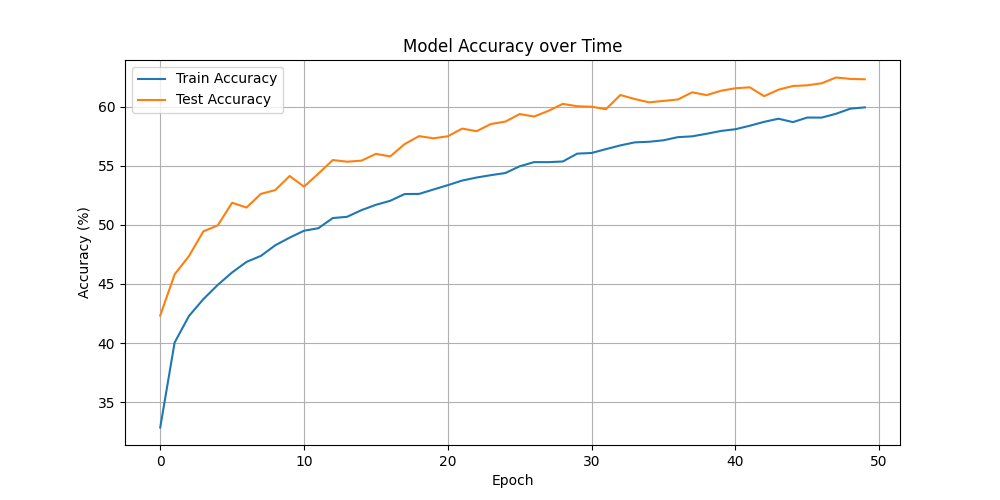
\includegraphics[width=0.5\textwidth]{media/cifar10_mlp_accuracy.png}
        \caption{MLP Accuracy History}
    \end{figure}
    \begin{figure}[H]
        \centering
        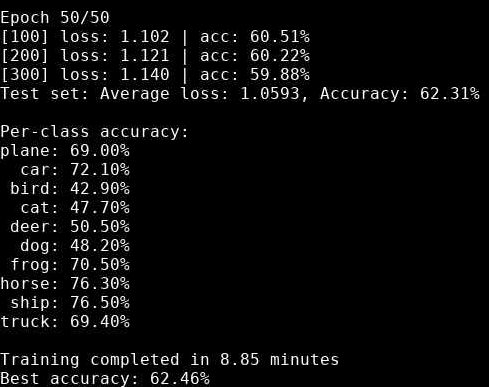
\includegraphics[width=0.5\textwidth]{media/mlp_epoch_50.png}
        \caption{MLP Epoch 50 Accuracy}
    \end{figure}
    \item \textbf{CNN:} They are composed of convolutional layers, pooling layers and fully connected
    layers. They are wired to understand spatial hierarchies in images using filters which scan the 
    entire image and detect patterns. It is mainly used for computer vision and is expect it of it
    to outperform the MLP model.
    \begin{figure}[H]
        \centering
        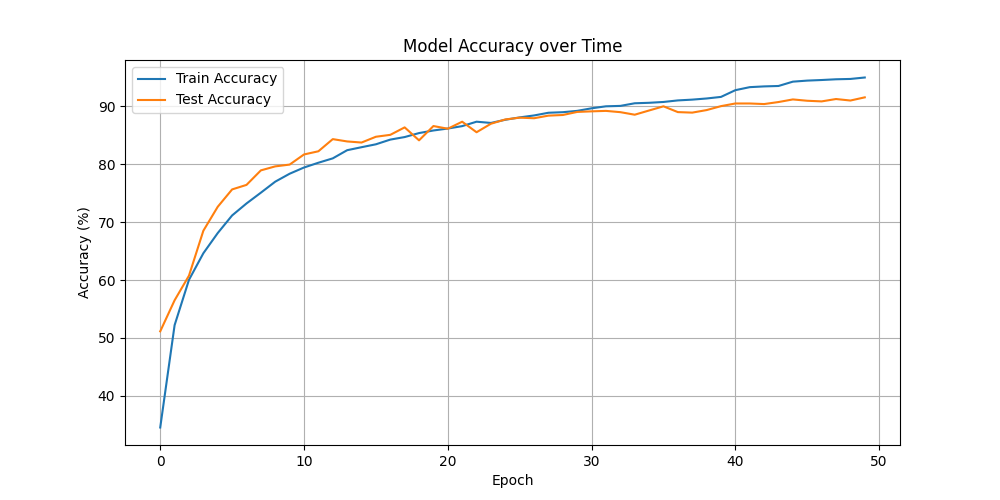
\includegraphics[width=0.5\textwidth]{media/cifar10_cnn_accuracy.png}
        \caption{CNN Accuracy History}
    \end{figure}
    \begin{figure}[H]
        \centering
        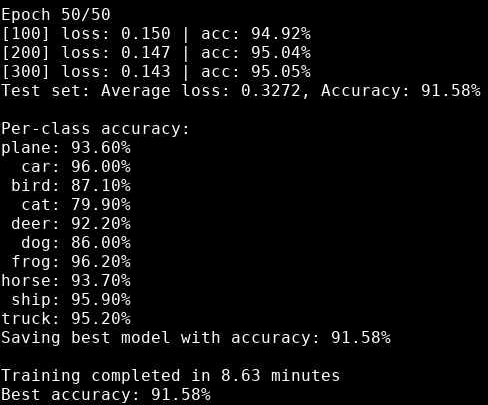
\includegraphics[width=0.5\textwidth]{media/cnn_epoch_50.png}
        \caption{CNN Epoch 50 Accuracy}
    \end{figure}
\end{itemize}

\subsection{Different Optimizer}
Here we are going to swap the Adam optimizer for the Stochastic Gradient Descent (SGD) optimizer.\\
\begin{itemize}
    \item \textbf{Adam:} It was our default optimizer on the CNN model. It is an algorithm which
    combines momentum and adaptive learning rates to converge faster. 
    \item \textbf{SGD:} Stochastic Gradient Descent is a simpler algorithm. Is exhibits fixed learning
    rate and is usually slower than Adam while also being less adaptive.
    \begin{figure}[H]
        \centering
        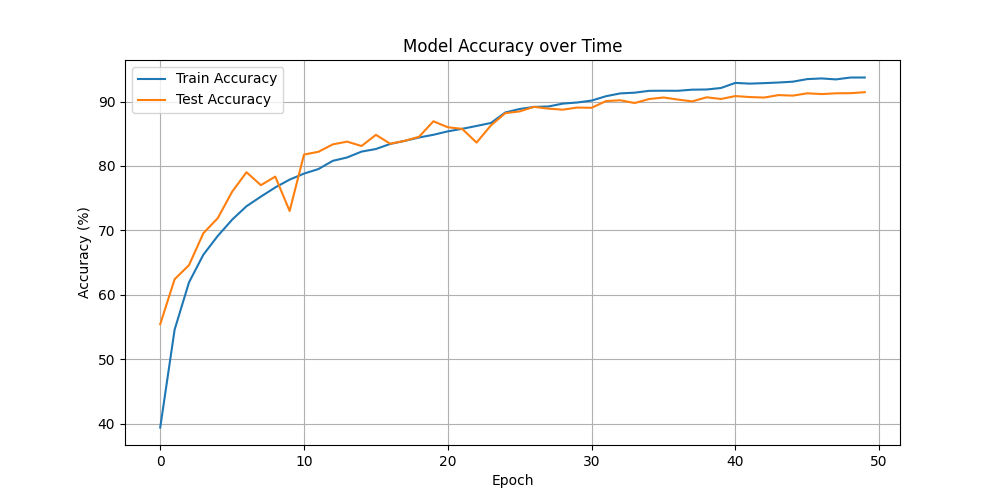
\includegraphics[width=0.5\textwidth]{media/cifar10_cnn_sgd_accuracy.png}
        \caption{SGD Accuracy History}
    \end{figure}
    \begin{figure}[H]
        \centering
        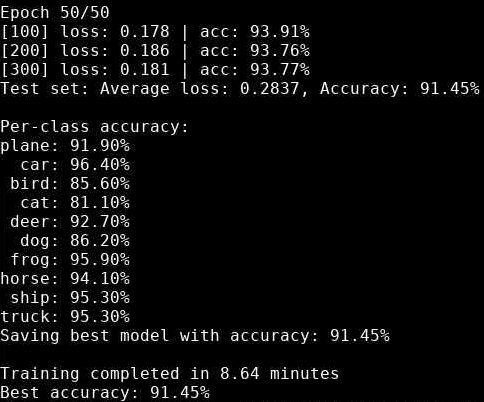
\includegraphics[width=0.5\textwidth]{media/cnn_sgd_epoch_50.png}
        \caption{SGD Epoch 50 Accuracy}
    \end{figure}
\end{itemize}

\subsection{Different Activation Functions}
Having used the ReLU activation function until now, it is time to test a different one. The one to 
fill its place will be the Tanh activation function.\\
\begin{itemize}
    \item \textbf{ReLU:} It was our default activation function on the CNN model. ReLU can be 
    defined by the mathematical expression $ f(x) = max(0,x) $. It outputs in the range $[0,\infty]$.
    \item \textbf{Tanh:} It is the tangent hyperbolic function 
    $$ tanh(x) = \frac{e^{x} - e^{-x}}{e^{x} + e^{-x}} $$.
    It is basically a sigmoid-shaped function that maps input values to the range [-1,1].
    \begin{figure}[H]
        \centering
        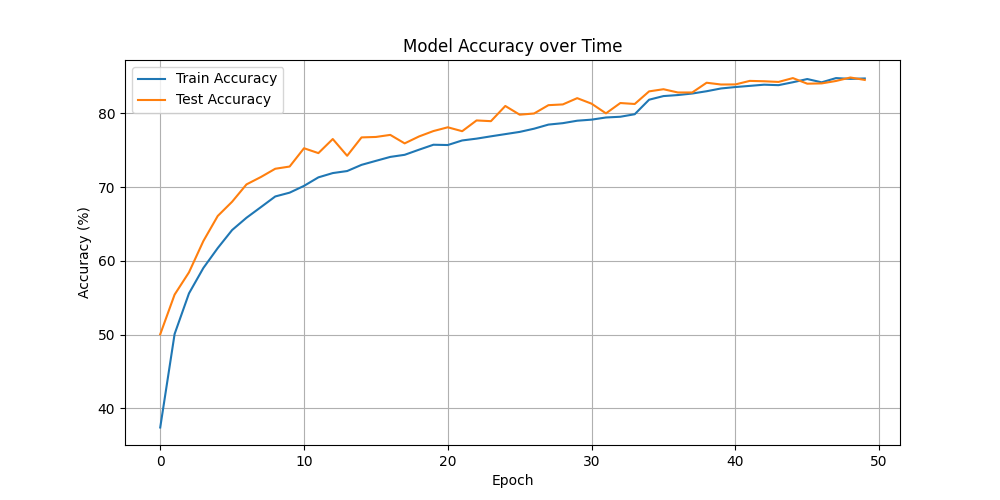
\includegraphics[width=0.5\textwidth]{media/cifar10_cnn_tanh_accuracy.png}
        \caption{Tanh Accuracy History}
    \end{figure}
    \begin{figure}[H]
        \centering
        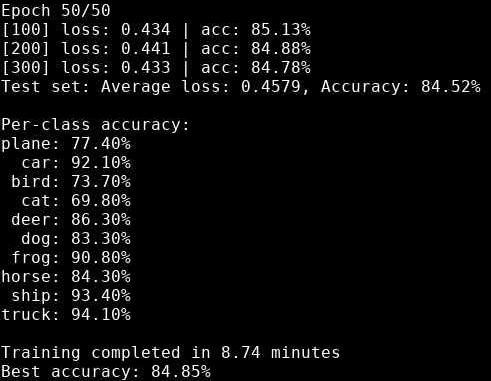
\includegraphics[width=0.5\textwidth]{media/cnn_tanh_epoch_50.png}
        \caption{Tanh Epoch 50 Accuracy}
    \end{figure}
\end{itemize}

\subsection{Different Normalization Values}
The last modification includes tinkering with different normalization values both for the mean and
the standard deviation.\\
\begin{itemize}
    \item \textbf{Default:} The default normalization values on the CNN model.
    \item \textbf{Standard [-1,1]:} It is identical to the default normalization values when it comes
    to the model's performance.
    \begin{figure}[H]
        \centering
        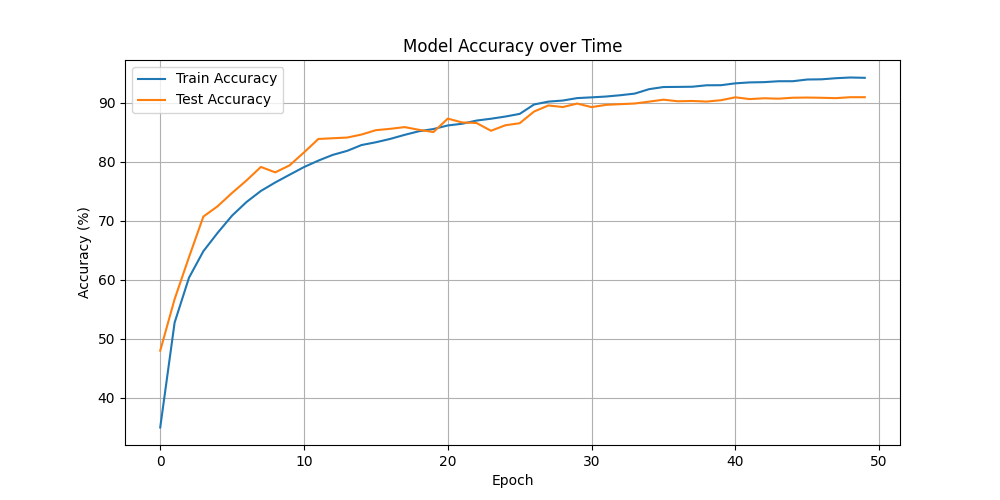
\includegraphics[width=0.5\textwidth]{media/cifar10_cnn_std_accuracy.png}
        \caption{Standard Normalization Accuracy History}
    \end{figure}
    \begin{figure}[H]
        \centering
        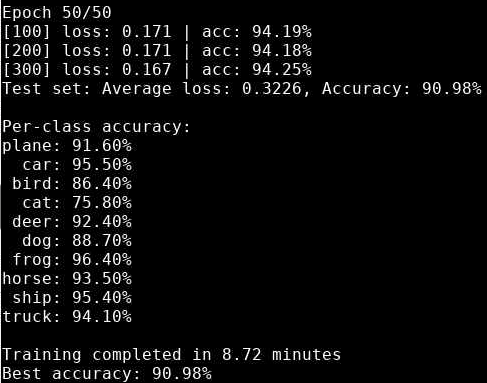
\includegraphics[width=0.5\textwidth]{media/cnn_std_epoch_50.png}
        \caption{Standard Normalization Epoch 50 Accuracy}
    \end{figure}
    \item \textbf{Zero-centered:} Same as the standard normalization values, there doesn't seem to be
    a significant difference. All normalization values had a very similar effect to the performance of
    the model.
    \begin{figure}[H]
        \centering
        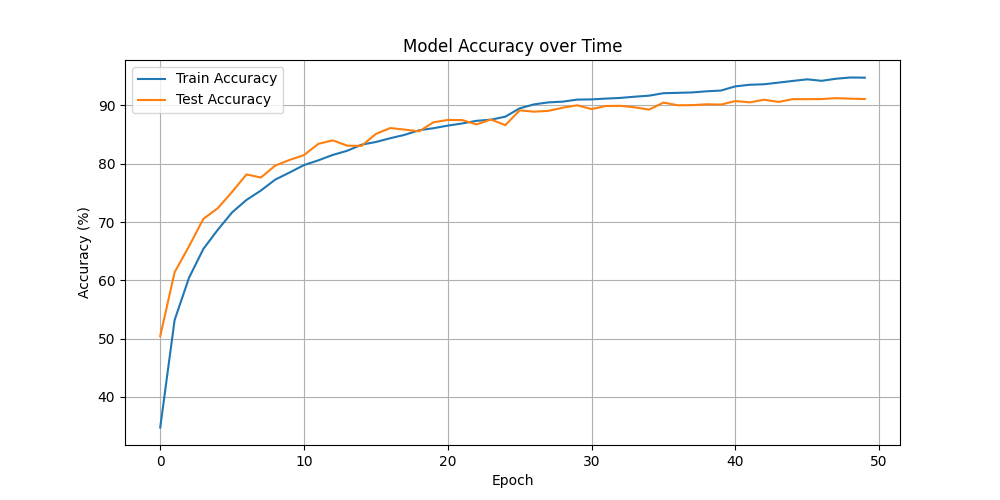
\includegraphics[width=0.5\textwidth]{media/cifar10_cnn_zero_accuracy.png}
        \caption{Zero-centered Normalization Accuracy History}
    \end{figure}
    \begin{figure}[H]
        \centering
        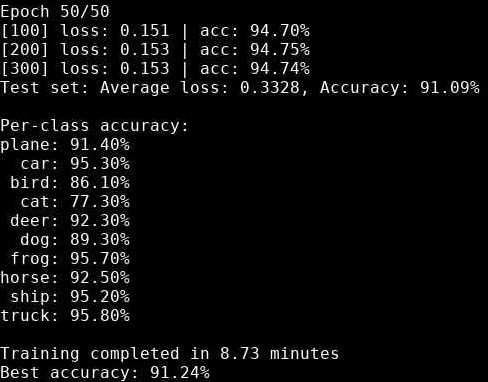
\includegraphics[width=0.5\textwidth]{media/cnn_zero_epoch_50.png}
        \caption{Zero-centered Normalization Epoch 50 Accuracy}
    \end{figure}
\end{itemize}
